\subsection{Bestimmung der Flächenträgheitsmomente}
Das Flächenträgheitsmoment ist eine Größe, die im weiteren Verlauf wichtig ist, um den Elastizitätsmodul der Stäbe zu ermitteln.
Er hängt vom Querschnitt des Stabes, genauer vom Abstand $y$ der Flächenelemente d$q$ zur neutralen Faser, ab
\begin{equation}
I = \int_{Q} y ^2 \, \text{d}q \quad .
\end{equation}
Für den eckigen Stab benötigt man eine Formel für quadratische Querschnitte. Nach den Werten aus Talbelle \ref{tab:querschnitte} ist mittlere Kantenlänge mit einem Ablesefehler von \SI{0.05}{\milli\metre}
\begin{align}
  h = \SI{0.01000 \pm 0.00005}{\metre}
\end{align}
ist das Flächenträgheitsmoment $I_\text{E}$
\begin{equation}
I_\text{E} = \int_{-\frac{h}{2}}^{\frac{h}{2}} \int_{-\frac{h}{2}}^{\frac{h}{2}} y^2\,  \text{d}x \text{d}y = \frac{1}{12} \cdot h^4 = \SI{3.88(17)e-10}{\metre^{4}} \quad .
\label{I_E}
\end{equation}
Um das Flächenträgheitsmoment für runde Querschnitte mit Radius $r$ zu berechnen, bietet sich die Verwendung von Polarkoordinaten an. Der Abstand zur $y$-Achse ist dann $r^2 \cdot \sin^2(x)$.  Mit der Jakobideterminante $r$. Der verwendete Radius aus Tablle \ref{tab:querschnitte} mit einem Ablesefehler von \SI{0.05}{\milli\metre} ist
\begin{equation}
  r = \SI{0.004975 \pm 0.000032}{\metre}
\end{equation}
und führ auf das Flächenträgheitsmoment
\begin{equation}
I_\text{R} = \int_{0}^{r}  \int_{0}^{2\pi} r^2 \cdot \sin^2(x) \cdot r  \, \text{d}\phi \text{d}r = \frac{1}{12}\cdot \pi \cdot r^4 = \SI{4.81(12)e-10}{\metre^{4}} \quad .
\label{I_R}
\end{equation}
\begin{center}
	\captionof{table}{Breite $h$ des eckigen Stabes und Durchmesser $2 \cdot r$ des Runden}
\begin{tabular}{c|c}
	Breite $h$ in \SI{}{\milli\metre}& Durchmesser $2 \cdot r$ in \SI{}{\milli\metre}	\\
	\hline
	10.00 & 10.00 \\
	10.00  & 10.00 \\
	10.00  & 10.00 \\
	10.00  & 9.90 \\
	10.00  & 9.90 \\
	10.00  & 9.95 \\
	10.00  & 10.00 \\
	10.00  & 9.90 \\
	10.00  & 9.90 \\
	10.00 & 9.95 \\
\end{tabular}	
\end{center}






\subsection{Bestimmung des Elastizitätsmoduls durch lineare Regression}
\subsubsection{Runder Stab -- einseitige Einspannung}
Die gemessene Durchbiegung $D(x)$ des Stabes wird durch Gleichung \eqref{einseitige Einspannung} beschrieben.
Alle in ihr vorkommende Größen, bis auf den Elastizitätsmodul sind bekannt. Das Flächenträgheitsmoment wurde im vorherigen Abschnitt in \eqref{I_R} bestimmt und die herabziehende Kraft $F$ ist aus der Masse des Probekörpers zu berechnen
\begin{equation}
  F = m \cdot g = \SI{0.7476}{\kilo\gram} \cdot \SI{9.81}{\metre\per\second\squared} = \SI{7.3339}{\newton} \quad .
\end{equation}
Nun lässt sich der Elastizitätsmodul $E$ durch eine lineare Regression der Form
\begin{equation}
  D(x) = \frac{F}{2\cdot E I}\left(Lx^2-\frac{x^3}{3}\right) = \frac{1}{E} \cdot A(x) +b
\end{equation}
bestimmen, indem $D(x)$ über $A(x)$ aufgetragen wird (siehe Abbildung \ref{fig:Regression_runder_Stab}). $E$ entspricht dann dem Kehrwert der Steigung der Regressionsgeraden. Unter Verwendung der Formeln aus Kapitel~\ref{sec:regression} ergeben sich die Steigung
\begin{equation}
  \frac{1}{E}= \SI{188.9(15)e-13}{\metre\squared\per\newton}
\end{equation}
und der $y$-Achsenabschnitt
\begin{equation}
  b = \SI{14.33(36)e-05}{\metre} \quad.
\end{equation}
Der gemessene Elastizitätsmodul für den runden Stab ist folglich
\begin{equation}
  E = \SI{5.29(4)e+10}{\newton\per\metre\squared} \quad.
\end{equation}

\begin{figure}
\centering
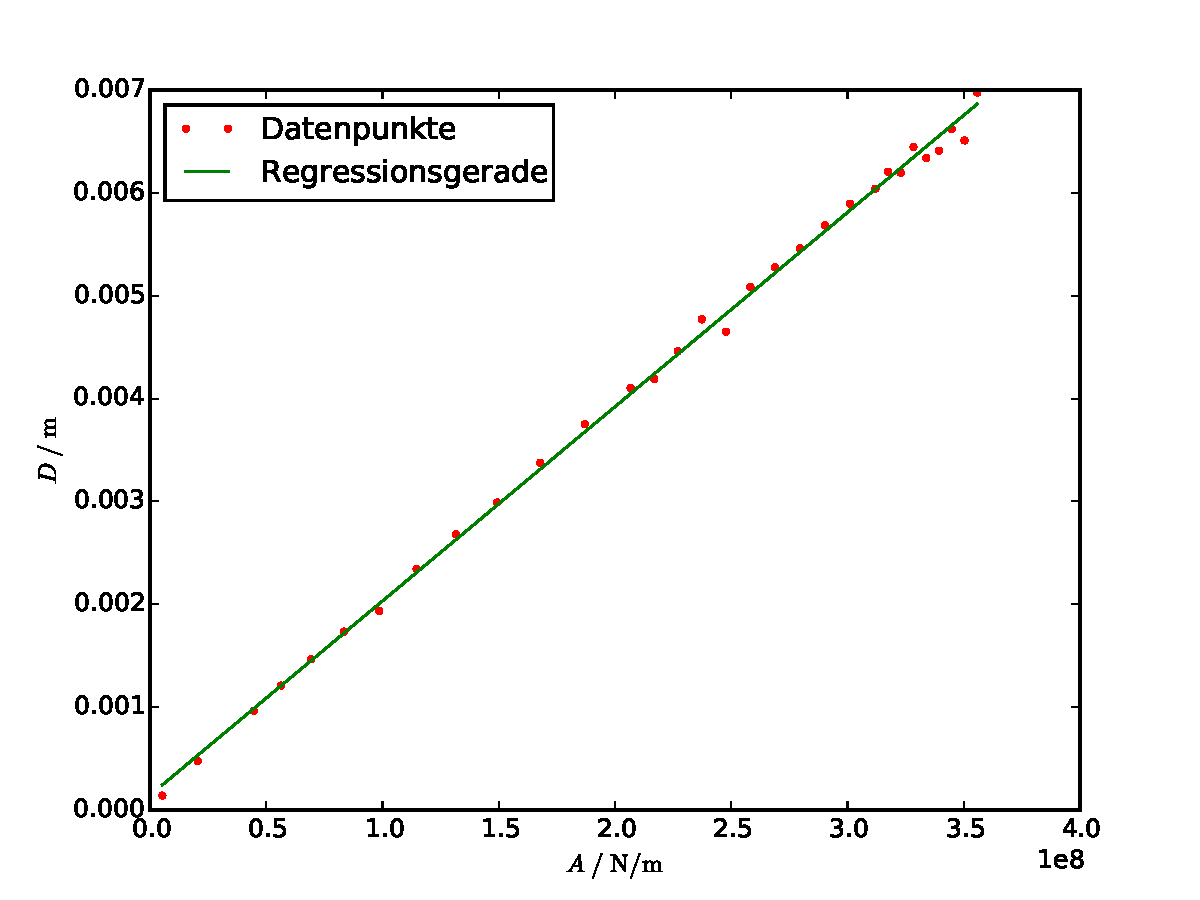
\includegraphics[width=\textwidth]{Regression_runder_Stab.pdf}
\caption{Regressionsgerade des runden Stabes bei einseitiger Einspannung}
\label{fig:Regression_runder_Stab}
\end{figure}



\subsubsection{Eckiger Stab -- einseitige Einspannung}
Hier ist der Vorgehensweise dieselbe, wie beim runden Stab. Es muss lediglich das Flächenträgheitsmoment aus \eqref{I_E} verwendet und die nach unten wirkende Kraft
\begin{equation}
  F = m \cdot g = \SI{0.7676}{\kilo\gram} \cdot \SI{9.81}{\metre\per\second\squared} = \SI{7.5302}{\newton}
\end{equation}
angepasst werden.
Dies führt zu einer Steigung von
\begin{equation}
  \frac{1}{E}= \SI{135.6(9)e-13}{\metre\squared\per\newton}
\end{equation}
und einem $y$-Achsenabschnitt
\begin{equation}
  b = \SI{6.28(217)e-05}{\metre} \quad.
\end{equation}
Der hier bestimmte Elastizitästmodul für den eckigen Stab ist demnach
\begin{equation}
  E = \SI{7.37(5)e+10}{\newton\per\metre\squared} \quad.
\end{equation}
Die Werte wurden in Abbildung~\ref{fig:Regression_eckiger_Stab} aufgetragen.

\begin{figure}[h!]
\centering
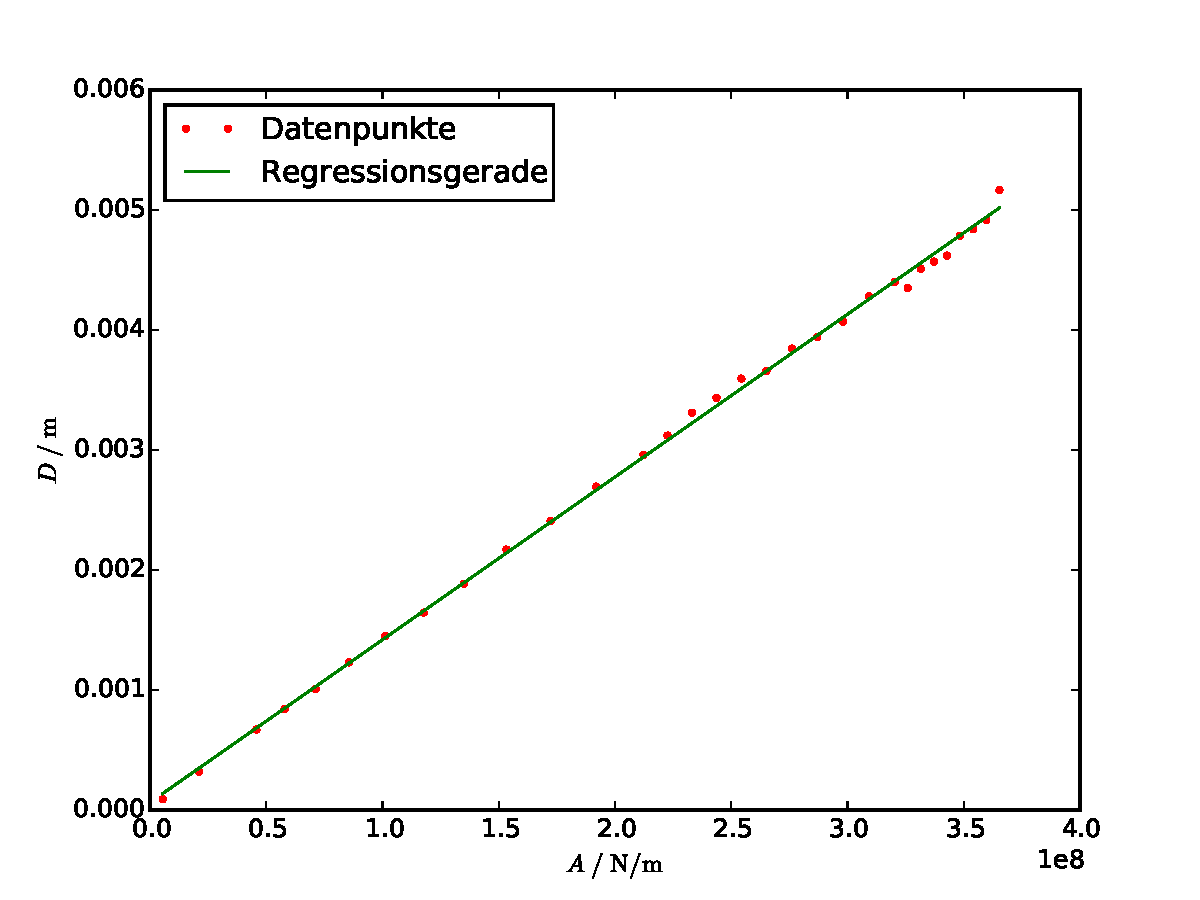
\includegraphics[width=\textwidth]{Regression_eckiger_Stab.pdf}
\caption{Regressionsgerade des eckigen Stabes bei einseitiger Einspannung}
\label{fig:Regression_eckiger_Stab}
\end{figure}







\subsubsection{Eckiger Stab -- beidseitige Einspannung}
Die Bestimmung des Elastizitätsmoduls bei beidseitiger Einspannung funktioniert analog. Es werden Formel \eqref{beidseitige Einspannung}
\begin{equation*}
	D(x) = \frac{F}{48\cdot E I}\left(3L^2x-4x^3\right) = \frac{1}{E}C(x)+b
\end{equation*}
und die eine herunterziehende Kraft von
\begin{equation}
  F = m \cdot g = \SI{4.7004}{\kilo\gram} \cdot \SI{9.81}{\metre\per\second\squared} = \SI{46.1109}{\newton}
\end{equation}
verwendet. \\
Da die Verbiegung des Stabes links und rechts der Mitte gemessen wurde, gibt es zwei Regressionsgeraden. \\
Zunächst soll die Regressionsgerade für die Werte der linken Seite (siehe Abbildung \ref{fig:linkeseite}) betrachtet werden. Sie hat eine Steigung von
\begin{equation}
  \frac{1}{E}= \SI{55.45(188)e-13}{\metre\squared\per\newton}
\end{equation}
und einen $y$-Achsenabschnitt von
\begin{equation}
  b = \SI{44.5(23)e-05}{\metre} \quad.
\end{equation}
Daraus folgt der Elastizitätsmodul
\begin{equation}
  E = \SI{18.0(6)e+10}{\newton\per\metre\squared} \quad.
\end{equation}
\\
Für die rechte Seite (siehe Abbildung \label{fig:rechteseite}) ergeben sich Werte von
\begin{align}
  \frac{1}{E} &= \SI{72.25(303)e-13}{\metre\squared\per\newton} \quad,\\
  b &= \SI{30.6(47)e-05}{\metre} \\
  \intertext{und}
  E &= \SI{13.8(6)e+10}{\newton\per\metre\squared} \quad.
\end{align}


\begin{figure}[h!]
\centering
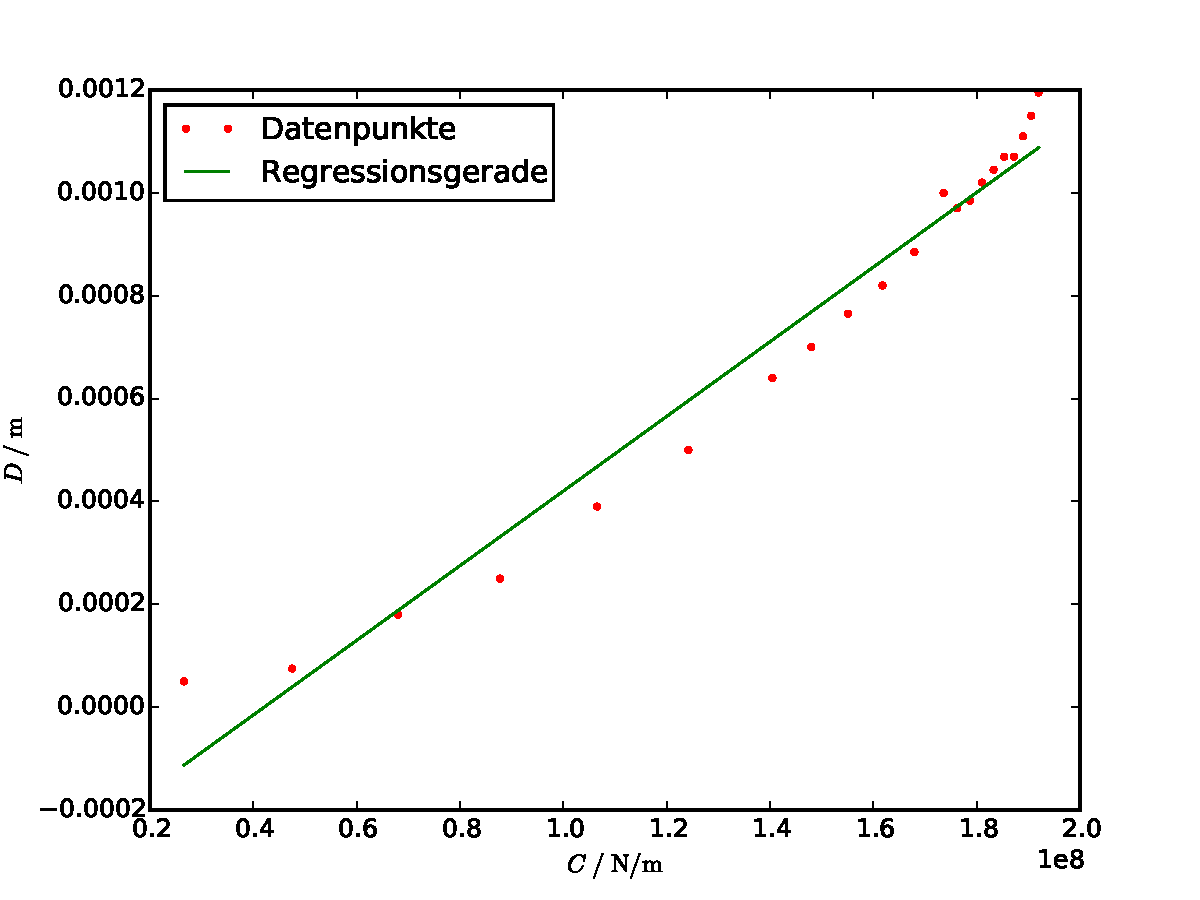
\includegraphics[width=\textwidth]{Regression_zweiseitig_eingespannt_1.pdf}
\caption{Regressionsgerade des eckigen Stabes bei beidseitiger Einspannung -- linke Seite}
\label{fig:linkeseite}
\end{figure}

\begin{figure}[h!]
\centering
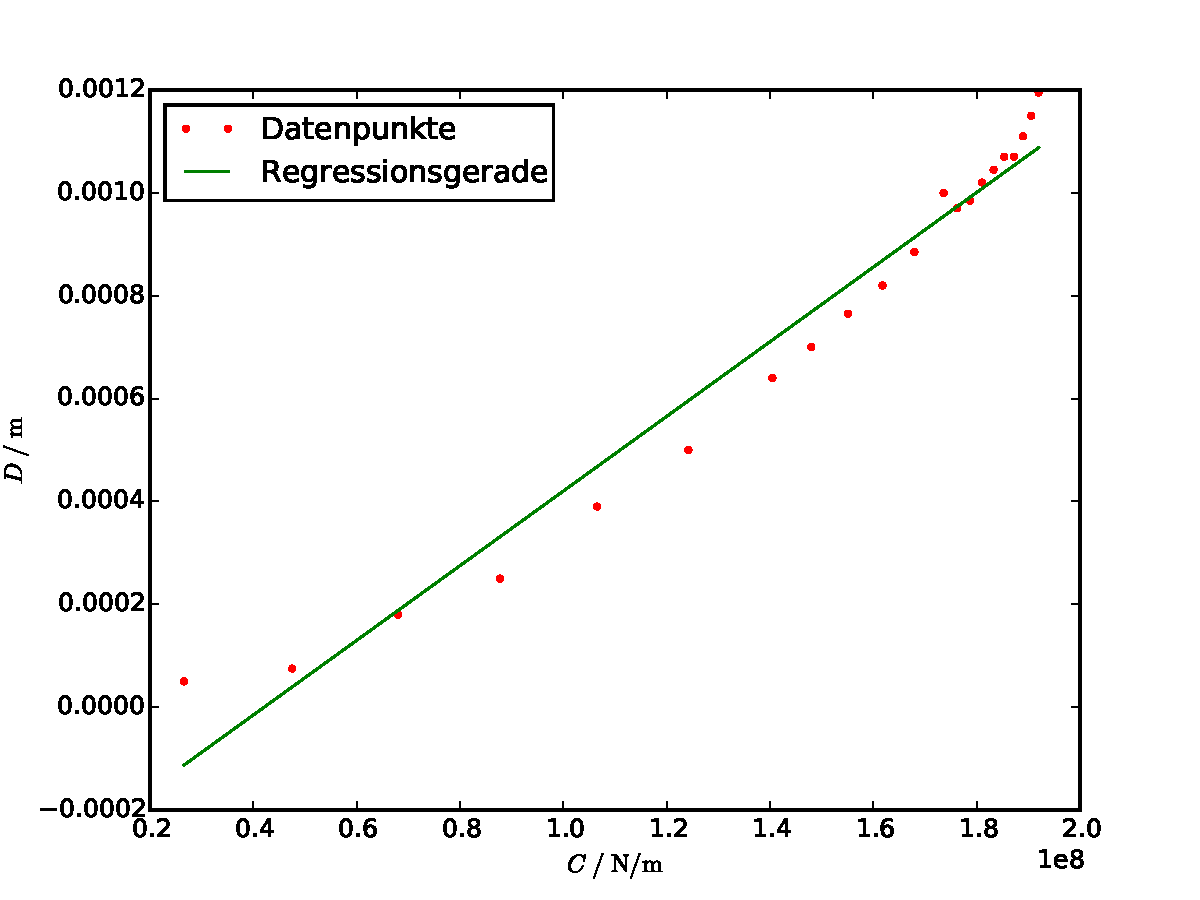
\includegraphics[width=\textwidth]{Regression_zweiseitig_eingespannt_2.pdf}
\caption{Regressionsgerade des eckigen Stabes bei beidseitiger Einspannung -- rechte Seite}
\label{fig:rechteseite}
\end{figure}



\subsection{Bestimmung der Dichte}
Mit der Dichte kann bestimmt werden, aus welchen Metallen die Stäbe bestehen. Um sie bestimmen zu können, wurden beide Stäbe vermessen und gewogen. Das Gewicht und die Länge sind keine fehlerbehafteten Größen. Der Durchmesser hingegen wurde mit einer Schieblehre mehrfach gemessen. Ein Ablesefehler von \SI{0.05}{\milli\metre}  kommt zum Fehler des Mittelwertes hinzu.
Der Querschnitt bzw. Radius der Stäbe wurde (Werte in Tabelle \ref{tab:querschnitte}) bereits als fehlerbehaftete Größe bestimmt. \\
Die Dichte ist jeweils
\begin{equation}
  \rho = \frac{\text{Gewicht}}{\text{Querschnittsfläche} \cdot \text{Länge}} \quad.
\end{equation}
Der runde Stab der Länge \SI{0.6}{\metre} ist \SI{0.3945}{\kilo\gram} schwer und hat die Dichte
\begin{equation}
  \rho_\text{Rund} = \SI{8455.90(10902)}{\kilo\gram\per\cubic\metre} \quad.
\end{equation}  \\
Und der eckige Stab der Länge \SI{0.6}{\metre} ist \SI{0.1671}{\kilo\gram} schwer und hat die Dichte
\begin{equation}
  \rho_\text{Eckig} = \SI{2785.00(2785)}{\kilo\gram\per\cubic\metre} \quad.
\end{equation}
